\textbackslash{}documentclass\{article\}

\section{Introduction}\label{introduction}

In this chapter I test the idea that the social science disciplines were
established in the United States in part through a process of cognitive
institutionalization. This means that the concept of each discipline
could not, especially early in its history, be taken for granted as
known or recognizable even among academics and intellectuals, not to
mention lay audiences. An impetus for the emergence of the disciplines
as professions was a dawning process of recognition of ``social
science'' problems or objects, followed by a consistent form of
categorizing the same.

To study such a process historically does not in the first instance
require an understanding of the objects that are categorized, and indeed
there is no requirement that the objects categorized are themselves
homogeneous. The act of labeling the world according to a convention can
attain a rigid consistency even if great doubt remains about the
meaning, significance, an coherence of the objects so organized.

Empirically, at least, in this study we do count the prevalance of
disciplinary terminology. How then can such terminology be counted? I
contend that a discipline is established as a categorization mechanism
when the set of possible labels for the same object shrinks to a short
and ranked list. The position at the top of that list will be occupied
by what we call the disciplinary prefix, and below it variations on
nouns used to capture different aspects of cultural content from created
work to the authors themselves.

\subsection{Genre}\label{genre}

Consider five social science disciplines--anthropology, economics,
political science, psychology, and sociology. In English the labels that
like flags lay claim to disciplinary territory are the prefixes soci-,
econ-, anth-, poli-, and psyc-. In the prehistory of disciplines these
stems appear as recognition of a category of phenomena that can be
talked about by anyone, long before a disciple existed to claim
priority.

These prefixes diffused first as weakly categorical terms that could
modify and lay claim to any worldly object. The first stem terms to
diffuse were generic modifiers like ``social'' and ``economic''. Such
labels, as ubiquitous and inexclusive as they were, defined the outer
limit of disciplinary relevance. The term ``social problem'' is an
example of the flag being established as a vague claim to disciplinary
relevance. Early in the history of disciplinary recognition, the
appelation of genre terms are little more than promises to demonstrate
that a problem is indeed a ``social'' one.

\begin{figure}

{\centering 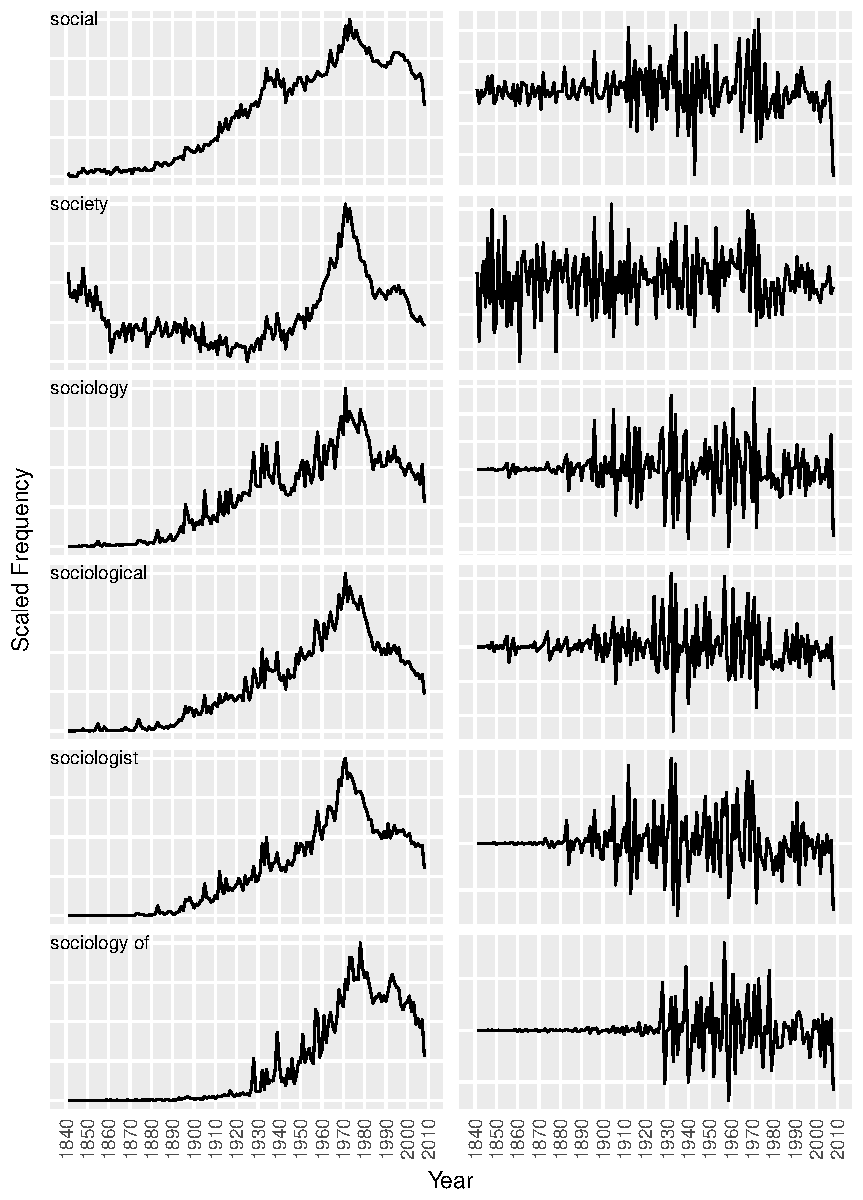
\includegraphics[width=\maxwidth]{~/prd/tex/fig/f-3prefix1-soci-1} 

}

\caption[Terms with Disciplinary Prefix soci-]{Terms with Disciplinary Prefix soci-}\label{fig:f-3prefix1-soci}
\end{figure}

\section{Temporal Sequencing Methods}\label{temporal-sequencing-methods}

Correlations between time series are difficult to tease out due to
several dynamics that if not controlled for can lead to spurious
correlations. Before we can attempt to test causal order we must
decompose historical trends in terms into their systematic and residual
components, such that we may test the residuals for patterns between two
series.

ARIMA models have been criticized for abstracting from historical
reality (Isaac and Griffin 1989:877). After establishing statistical
considerations and laying bare our assumptions, we will discuss the
historical and ontological limitations of the statistical approach.

\subsection{Series}\label{series}


\begin{table}[!htbp] \centering 
  \caption{Terms searched in the Google Books Ngrams Database} 
  \label{query} 
\begin{tabular}{@{\extracolsep{5pt}} llllll} 
\\[-1.8ex]\hline 
\hline \\[-1.8ex] 
& soci & econ & anth & poli & psyc \\ 
\hline \\[-1.8ex] 
Genre & social & economic & cultural & political & mental \\ 
Technique & sociological & economical & anthropological & political & psychological \\ 
Ontology & society & economy & culture & polity & mind \\ 
Discipline & sociology & economics & anthropology & political science  & psychology \\ 
Profession & sociologist & economist & anthropologist & political scientist & pscyhologist \\ 
Subdiscipline & sociology of & economics of & anthropology of & political science of & psychology of \\ 
\hline \\[-1.8ex] 
\end{tabular} 
\end{table} 

\subsection{ARIMA model}\label{arima-model}

ARIMA, or Auto Regressive Integrated Moving Average, models are
effective in decomposing several categories of within-series
correlations.

\begin{equation}
\text{I} = \frac{\text{MA}}{\text{AR}}
\end{equation}

This says that \(I\), the change in our series, is a function of \(MA\),
a moving but systematic average (a line or higher order polynomial) and
\(AR\), the value of the difference in one or more preceding time steps.
In more detail:

\begin{equation}
 (1-B)^d y_{t} = \frac{c + (1 + \theta_1 B + \cdots + \theta_q B^q)e_t}{(1-\phi_1B - \cdots - \phi_p B^p)}
\end{equation}

Where \(c\) is a constant drift up or down, \(theta\), \(phi\),
\(y_{t}\), \(d\), \(q\), \(p\), and \(e_t\). \(B\).

\subsection{Granger Causality}\label{granger-causality}

What is the temporal sequence of these terms in each discipline?

\section{Results}\label{results}

As table \ref{t-prefix} shows.

\section{Which came first?}\label{which-came-first}

Granger tests can help determine which (Thurman and Fisher 1988; Granger
1969)

Clear secular trends and period effects surrounding WWII and the baby
boom. To control:

\begin{itemize}
\tightlist
\item
  Model the trends. We could estimate the linear trend or splines and
  then subtract them.
\item
  First differences. Subtract from each point the previous point.
\item
  Link relatives. Divide each point from the point before it.
\end{itemize}

Box Cox doesn't mean

\begin{equation}\tag{8.1}\label{eq-8-arima} y'_{t} = c +
\phi_{1}y'_{t-1} + \cdots + \phi_{p}y'_{t-p} +
\theta_{1}e_{t-1} + \cdots + \theta_{q}e_{t-q} + e_{t},
\end{equation}

\section*{References}\label{references}
\addcontentsline{toc}{section}{References}

\hypertarget{refs}{}
\hypertarget{ref-Granger:1969wx}{}
Granger, C W J. 1969. ``Investigating Causal Relations by Econometric
Models and Cross-spectral Methods.'' \emph{Econometrica} 37 (3): 424.

\hypertarget{ref-Isaac:1989hp}{}
Isaac, Larry W, and Larry J Griffin. 1989. ``Ahistoricism in Time-Series
Analyses of Historical Process: Critique, Redirection, and Illustrations
from U.S. Labor History.'' \emph{American Sociological Review} 54 (6):
873.

\hypertarget{ref-Thurman:1988va}{}
Thurman, Walter N, and Mark E Fisher. 1988. ``Chickens, Eggs, and
Causality, or Which Came First?'' \emph{American Journal of Agricultural
Economics} 70 (2): 237.
